\documentclass{beamer}

\usepackage{beamerthemesplit}
\usepackage{verbatim}
\usepackage[normalem]{ulem}

\usepackage{xcolor}

\usepackage{hyperref}

\definecolor{gold}{rgb}{1.,0.84,0.}
\definecolor{brightred}{rgb}{1.,0.4,0.4}
\definecolor{mygray}{RGB}{200,200,200}
\definecolor{lightsteelblue}{RGB}{176,196,222}
\definecolor{lightskyblue}{RGB}{135,206,250}
\definecolor{cadetblue}{RGB}{95,158,160}

\usetheme{default}
\usecolortheme{mule}

\usefonttheme{serif}

%\DeclareGraphicsExtensions{.pdf,.png,.jpg}

\newcommand{\mcal}{\textsc{metacalibration}}
\newcommand{\Mcal}{\textsc{Metacalibration}}

\newcommand{\mcalR}{\mbox{\boldmath $R$}}
\newcommand{\mcalRscalar}{\mbox{$R$}}

\newcommand{\mcalRmean}{\mbox{\boldmath $\langle R \rangle$}}
\newcommand{\mcalRscalarmean}{\mbox{$\langle R \rangle$}}

\newcommand{\mcalRpsf}{$R^{p}$}
\newcommand{\mcalRpsfnoise}{$R^{p}_\eta$}
\newcommand{\mcalRo}{\mbox{\boldmath $R_o$}}
\newcommand{\mcalRnoise}{\mbox{\boldmath $R_\eta$}}

\newcommand{\mcalRmeanalpha}{\mbox{\boldmath $\langle R_\alpha \rangle$}}
\newcommand{\mcalRmeanbeta}{\mbox{\boldmath $\langle R_\beta \rangle$}}

\newcommand{\mcalRg}{\mbox{\boldmath $R_\gamma$}}
\newcommand{\mcalRS}{\mbox{\boldmath $R_S$}}
\newcommand{\mcalRgmean}{\mbox{\boldmath $\langle R_\gamma \rangle$}}
\newcommand{\mcalRSmean}{\mbox{\boldmath $\langle R_S \rangle$}}

\newcommand{\mcalRtwopt}{\mbox{\boldmath $R^{2pt}$}}
\newcommand{\mcalRtwoptmean}{\mbox{\boldmath $\langle R^{2pt} \rangle$}}


\newcommand{\mcalRmodel}{\mbox{\boldmath $R^{model}$}}
\newcommand{\mcalRnoisemodel}{\mbox{\boldmath $R^{model}_\eta$}}


\newcommand{\vecg}{\mbox{\boldmath $\gamma$}}
\newcommand{\vest}{\mbox{\boldmath $e$}}

\newcommand{\snr}{$S/N$}
\newcommand{\snT}{$(S/N)_{\textrm{size}}$}
%\newcommand{\snT}{$\left( \frac{S}{N}\right)_{\textrm{size}}$}
\newcommand{\snflux}{$(S/N)_{\textrm{flux}}$}
%\newcommand{\snflux}{$\left( \frac{S}{N}\right)_{\textrm{flux}}$}

\newcommand{\lensfit}{\texttt{LENSFIT}}
\newcommand{\numba}{\texttt{Numba}}
\newcommand{\python}{\texttt{Python}}
\newcommand{\ngmix}{\texttt{ngmix}}
\newcommand{\ngmixer}{\texttt{ngmixer}}
\newcommand{\shear}{{\bf g}}
\newcommand{\redmapper}{redMaPPer}
\newcommand{\est}{$e$}


\newcommand{\prelim}{{\bf{\it Preliminary}}}

\newcommand{\uberseg}{{\color{lightsteelblue} {\"u}berseg}}
\newcommand{\MOF}{{\color{brightred}MOF}}


\title{New MOF Deblender Implementation}
\author{Erin Sheldon}
\institute{Brookhaven National Laboratory}

% http://texblog.net/latex-archive/plaintex/beamer-footline-frame-number/
% to add the page (frame ) number and not screw up the bottom line
% works for split themes?
\expandafter\def\expandafter\insertshorttitle\expandafter{%
      \insertshorttitle\hfill%
        \insertframenumber\,/\,\inserttotalframenumber}

% suppress navigation bar
\beamertemplatenavigationsymbolsempty
\setbeamertemplate{footline}{}

\begin{document}


\frame{\titlepage}




\frame
{
    \frametitle{Original Multi-object Fitting}

    \begin{itemize}

        \item Idea to simultaneously fit all objects in a blend to 
            flexible models using \ngmix.

        \item Wanted to use full bulge+disk, but I found a this fit to be
            unstable. Adopted an SDSS-style composite model.  Fit bugle and
            disk models separately, then combine to a single model and re-fit.

        \item Not possible with composite model to do full simultaneous fit of
            all objects.  Matt adopted iterative method:  fit each object
            separately, subtracting light from neighbors.  Repeat until the
            system converges.
            
        \item Each object fitted on average about 12 times, to 3 different
            models!

    \end{itemize}

}

\frame
{
    \frametitle{Stable Bulge+Disk Model}

    \begin{itemize}

        \item I found the following to provide a stable fit, with
            enough flexibility for most purposes:

        \item Fix size $T$ of bulge and disk to be equal.  Make
            bulge and disk co-centric and co-elliptical.

        \item Place a simple gaussian prior on fraction of light
            in Bulge \texttt{fracdev}, centered at zero (pure disk).

        \item Informative prior on the ellipticity.  Uninformative
            priors on size and flux.  Moderately informative prior
            on center (informative for close blends).

        \item At high S/N can describe most galaxies fairly well.
            
        \item At low S/N provides a stable fit. Because most low S/N galaxies
            are also small compared to the PSF, adequate description of the
            observed light profile.

    \end{itemize}

}

\frame
{
    \frametitle{Full Multi-object Fitting}

    \begin{itemize}

        \item Take detections and starting points for
            center, size, and flux from Source Extractor.  Use the
            above listed priors.
            
        \item Can fit large groups simultaneously.

        \item In simulations, very stable, sub-percent failure rate
            even for large groups.

        \item I have fitted up to 225 objects (all of the 24 such groups I tried converged
            in about 75 minutes).


    \end{itemize}

}
\frame
{
    \frametitle{Advantages of this approach}

    \begin{itemize}

        \item Should be 4-5 times faster than the iterative approach

        \item The fitting is ``atomic''.  The entire group succeeds or fails.

        \item Better parameter covariance matrix for each object.

        \item We get some covariance information between objects.

    \end{itemize}
}

\frame
{
    \frametitle{Example Deblend}

        256 objects, 220 found by SExtractor
    \begin{center}
        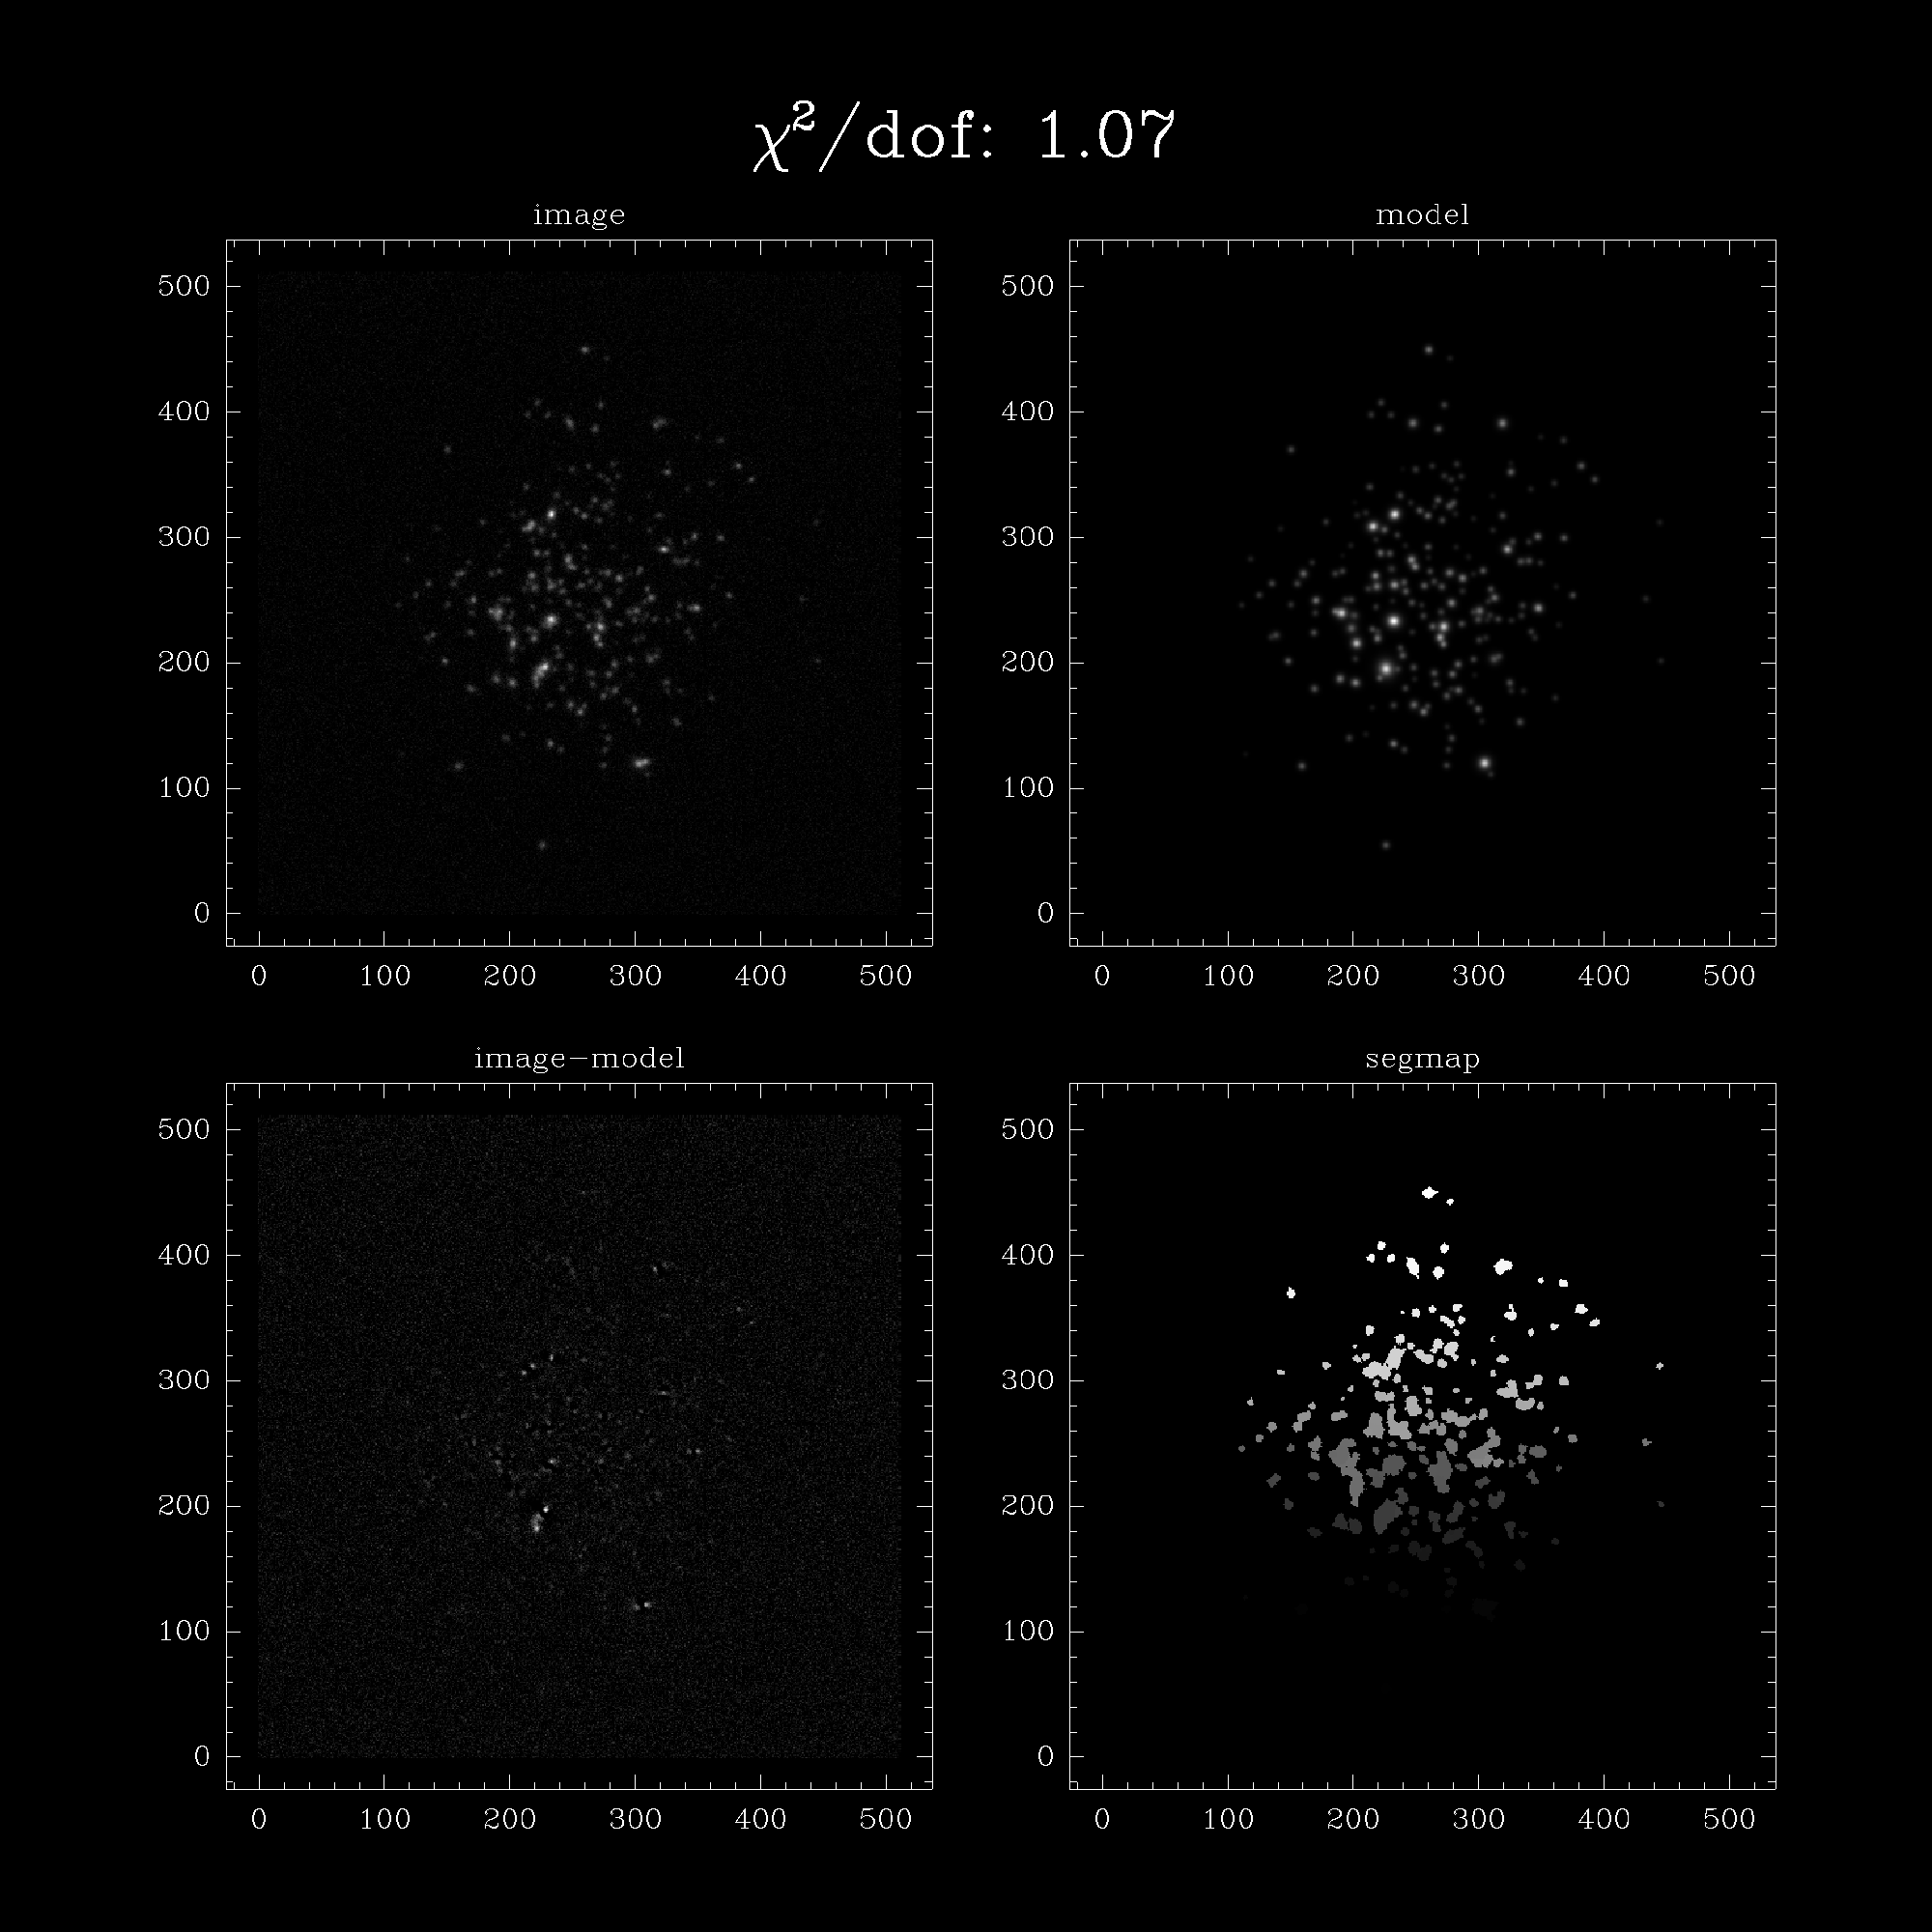
\includegraphics[width=0.7\columnwidth]{diff-20855-000000.png}
    \end{center}
}

\frame
{
    \frametitle{Example Deblend}

        256 objects, 220 found by SExtractor
    \begin{center}
        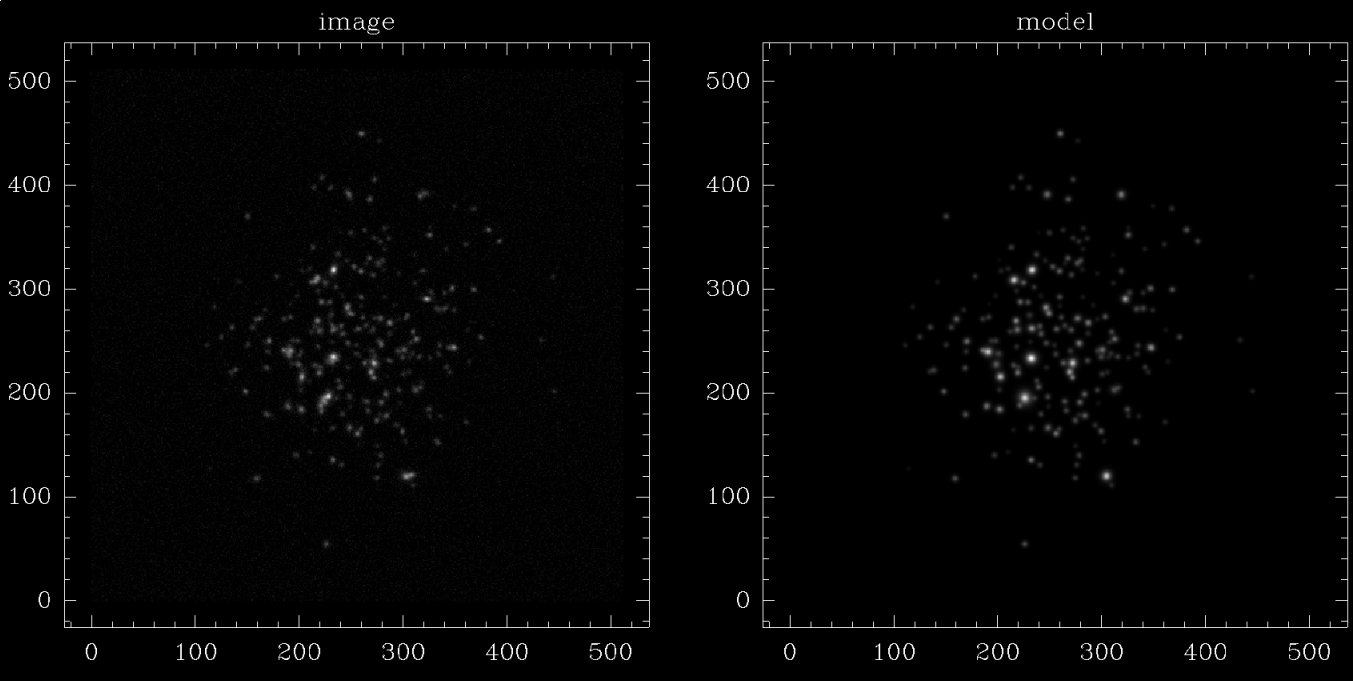
\includegraphics[width=\columnwidth]{example-side-by-side.png}
    \end{center}
}




\frame
{
    \frametitle{Crowded field problems}

    \begin{itemize}

        \item I fit a simple exponential disk and got very similar residuals

        \item The dominant problem in crowded regions is detection.

    \end{itemize}
}

\frame
{
    \frametitle{Shear tests}

    See the later talk about shear tests of the new MOF and the Scarlet deblender
}


%\frame
%{
%    \frametitle{\mcal\ PSF leakage}

%    \begin{center}
%        \includegraphics[width=0.9\columnwidth]{{y3v02-mcal-001-e-vs-epsf0-s2n-10.0-Tratio-0.50}.pdf}
%    \end{center}
%}


\end{document}
